%%%%%%%%%%%%%%%%%%%%%%%%%%%%%%%%%%%%%%%%%%%%%%%%%%%%%%%%%%%%%%%%%%% 
%                                                                 %
%                            CHAPTER                              %
%                                                                 %
%%%%%%%%%%%%%%%%%%%%%%%%%%%%%%%%%%%%%%%%%%%%%%%%%%%%%%%%%%%%%%%%%%% 

\chapter{Setting aanval}\label{chap:inferentieaanval}
In dit hoofdstuk beschrijven we de setting alsook de werking van de aanval. De
aanval is sterk gebaseerd op de aanvallen van~\citeauthor{Dhondt}
en~\citeauthor{Verdonck_2022}~\cite{Verdonck_2022, Dhondt}. Deze aanvallen
worden inferentieaanvallen genoemd, vanwege het feit dat uit metadata
essentiële gegevens kunnen worden geïnfereerd. In het geval
van~\citeauthor{Dhondt} gaat dit over afgelegde afstand binnenin de \ac{EPZ}.
In het geval van~\citeauthor{Verdonck_2022} gaat dit dan weer over geïnduceerde
hoogteverschillen binnen de privacy zone. Allereerst zullen we kort de
mogelijkheden van een aanvaller in de huidige setting bespreken. Daarna wordt
de inferentieaanval van~\citeauthor{Dhondt}, die de basis vormt voor de aanval
in deze thesis, besproken volgens een opdeling in drie stappen.

\section{Definitie aanvaller}\label{sec:definitie-aanvaller}
Deze thesis voert een onderzoek naar de mogelijkheid om een \ac{EPZ} te
omzeilen. De studie wordt dus gevoerd vanuit het opzicht van een aanvaller.
Vooraleer we de werking van een aanval kunnen beschreven, is het belangrijk om
een zicht te hebben op het doel en de capaciteiten van een aanvaller.

Hier is een aanvaller een gebruiker van het platform die geen eigenaar is van
een activiteit. Hij heeft echter wel zicht op alle metadata die publiekelijk
gedeeld is. Dit is data zoals afgelegde afstand, snelheid, tempo, \ldots \
Aangezien de aanval gaat over het omzeilen van \acp{EPZ} worden enkel
activiteiten beschouwd die gecloaked zijn. De aanvaller heeft dus geen zicht op
de reële start- en/of eindlocatie. Zijn of haar doel is dan ook om ondanks de
aanwezigheid van cloaking deze gevoelige locatie te achterhalen.

Vanuit het oogpunt van de inferentieaanval beschreven door~\citeauthor{Dhondt}
heeft de aanvaller toegang tot alle data die publiek beschikbaar is. In deze
aanval wordt echter wel voornamelijk gebruik gemaakt van afstandsdata. De
aanvaller die we in deze thesis beschrijven, heeft echter geen toegang tot deze
afstandsdata. Hij heeft wel nog toegang tot de ruwe gps-data, maar ook de
snelheid, het tempo enzovoort. Het onderzoek bestaat er dus uit om te zien in
hoeverre een aanval nog mogelijk is wanneer de afstandsdata onbruikbaar zou
zijn. We onderzoeken dus een alternatieve aanpak om de inferentieaanval alsnog
succesvol te kunnen uitvoeren.

We beschrijven de aanvaller vanuit een theoretisch kader. We bestuderen onder
welke omstandigheden de aanval mogelijk is, en welke maatregelen effectief
blijken. Het globale scenario waar we van uitgaan is: `wat als fitnesstrackers
de afstandsgegevens op een bepaalde manier zouden verbergen of onbruikbaar
maken, door bijvoorbeeld afrondingen te maken, of onzekerheid toe te voegen'.
Is de aanval dan nog mogelijk, en zo ja, hoe effectief is deze dan nog, en wat
voor gevolgen heeft dit ten opzichte van eerder bespoken
beschermingsmaatregelen?

\subsection{Assumpties}\label{sec:assumpties}
Om de aanval te kunnen uitvoeren, moeten enkele assumpties worden gemaakt.
\citeauthor{Dhondt} maakten al enkele assumpties om de inferentieaanval
succesvol uit te voeren. Voor dit onderzoek is het dus logisch om dezelfde
veronderstellingen te maken. Zo kunnen we een nuttige vergelijking maken. De
eerste assumptie stelt dat de zichtbare begin -en eindpunten op de rand van de
\ac{EPZ} moeten liggen. Ten tweede moet de beschermde locatie op de roadgraph
liggen. Hij kan niet buiten het voor ons te mappen gebied liggen, bijvoorbeeld
in een bos waar geen pad in kaart is gebracht. Er wordt dieper ingegaan op de
roadgraph in Sectie~\ref{sec:roadgraph}. Als laatste, maar desalniettemin
belangrijk punt moet de gebruiker binnenin de \ac{EPZ} de kortste route
volgen~\cite{Dhondt}.

Dhondt et al.\ maakte nog een laatste assumptie betreffende start- en
eindpunten, meer bepaald dat deze die dezelfde locaties moeten voorstellen. Dit
is echter niet van toepassing op dit onderzoek. Het onderzoek focust zich op
activiteiten waar slechts één deel van het traject verborgen is. Dit wil dan
ook zeggen dat de gebruiker ofwel vertrekt op de gevoelige locatie, of er
eindigt, maar niet beide. Op Figuur~\ref{fig:totalDistanceAttack} zijn de 2
mogelijke scenarios van een total distance attack terug te vinden, namelijk
waarbij ofwel gestart als geëindigd wordt binnenin de zone. Dit wordt ook een
\textit{total distance attack} genoemd, omdat enkel de totale afstand en de
afstand buiten de \ac{EPZ} nodig is. Op deze figuur zijn de rode punten
gelabeld \textit{Start} en \textit{End} de zichtbare start- en eindpunten. Dit
scenario stelt dat één van de reële start- of eindpunten de gevoelige locatie
is, aangeduid met de zwarte markering. Een andere aanval is de \textit{inner
    distance attack}, hierbij zullen zowel de start als het einde van een
activiteit binnenin het te verbergen gebied liggen, dit is te zien op
Figuur~\ref{fig:innerDist}. De kennis van de afzonderlijke afstand die de
gebruiker aflegt van de effectieve startlocatie tot de rand van de \ac{EPZ} en
van de rand van de \ac{EPZ} tot de effectieve eindlocatie is dan ook een
vereiste. Op de Figuur zijn opnieuw de zichtbare randpunten aangeduid in het
rood. Echter zal het onzichtbare traject voor beide gevallen doorlopen en
eindigen op de gevoelige locatie, wat in dit geval de reële start- en
eindlocatie is. In Sectie~\ref{sec:berekeningen} wordt dieper ingegaan op de
reden waarom een \textit{inner distance attack} niet mogelijk is. In deze
thesis worden dus alle activiteiten waarvan enkel een verhulde start- of
eindlocatie behouden, de rest wordt gefilterd in deze context.
\begin{figure}[h]
    \centering
    \begin{subfigure}[b]{.5\textwidth}
        \centering
        \caption{Start binnenin de \ac{EPZ}}
        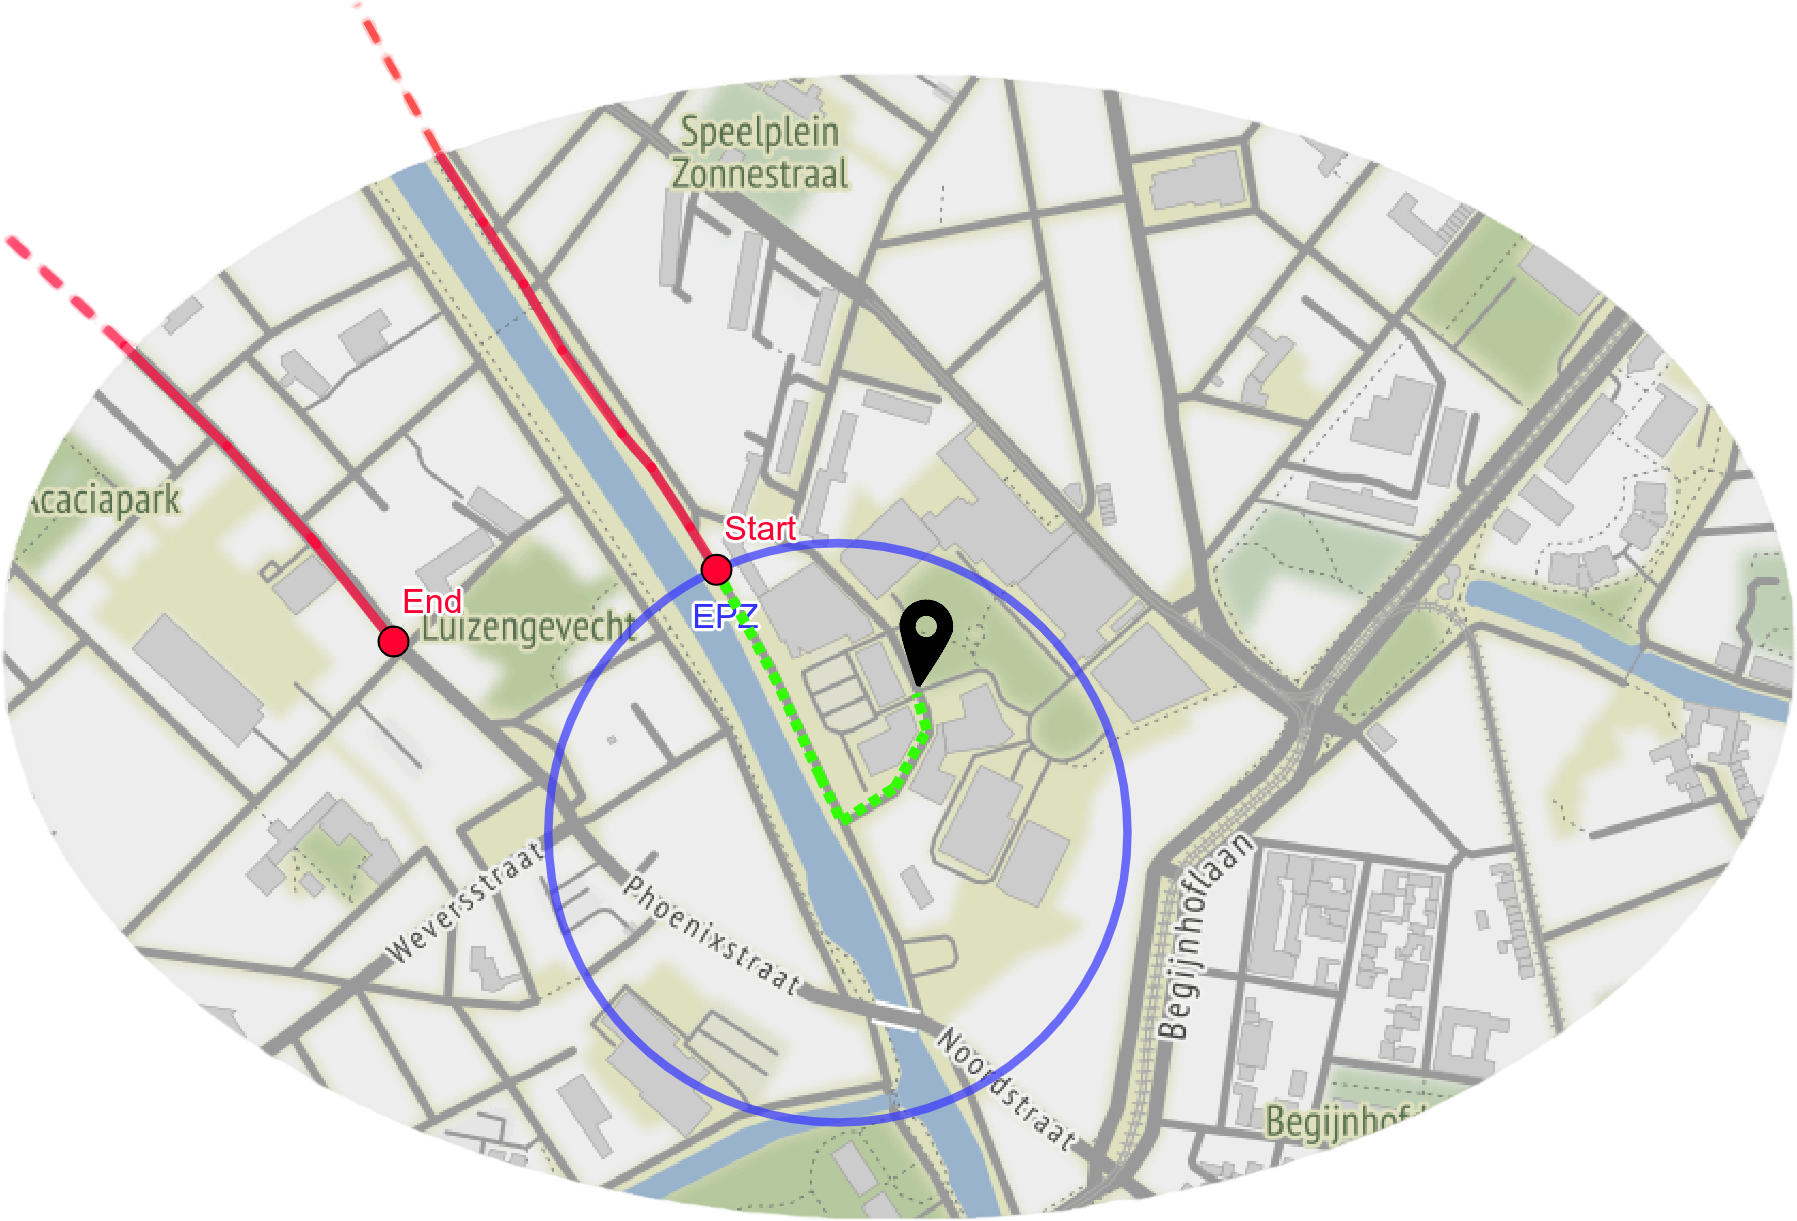
\includegraphics[width=1\textwidth]{fig/TotalDistanceAttacks/start.png}
    \end{subfigure}\hfill
    \begin{subfigure}[b]{.5\textwidth}
        \centering
        \caption{Einde binnenin de \ac{EPZ}}
        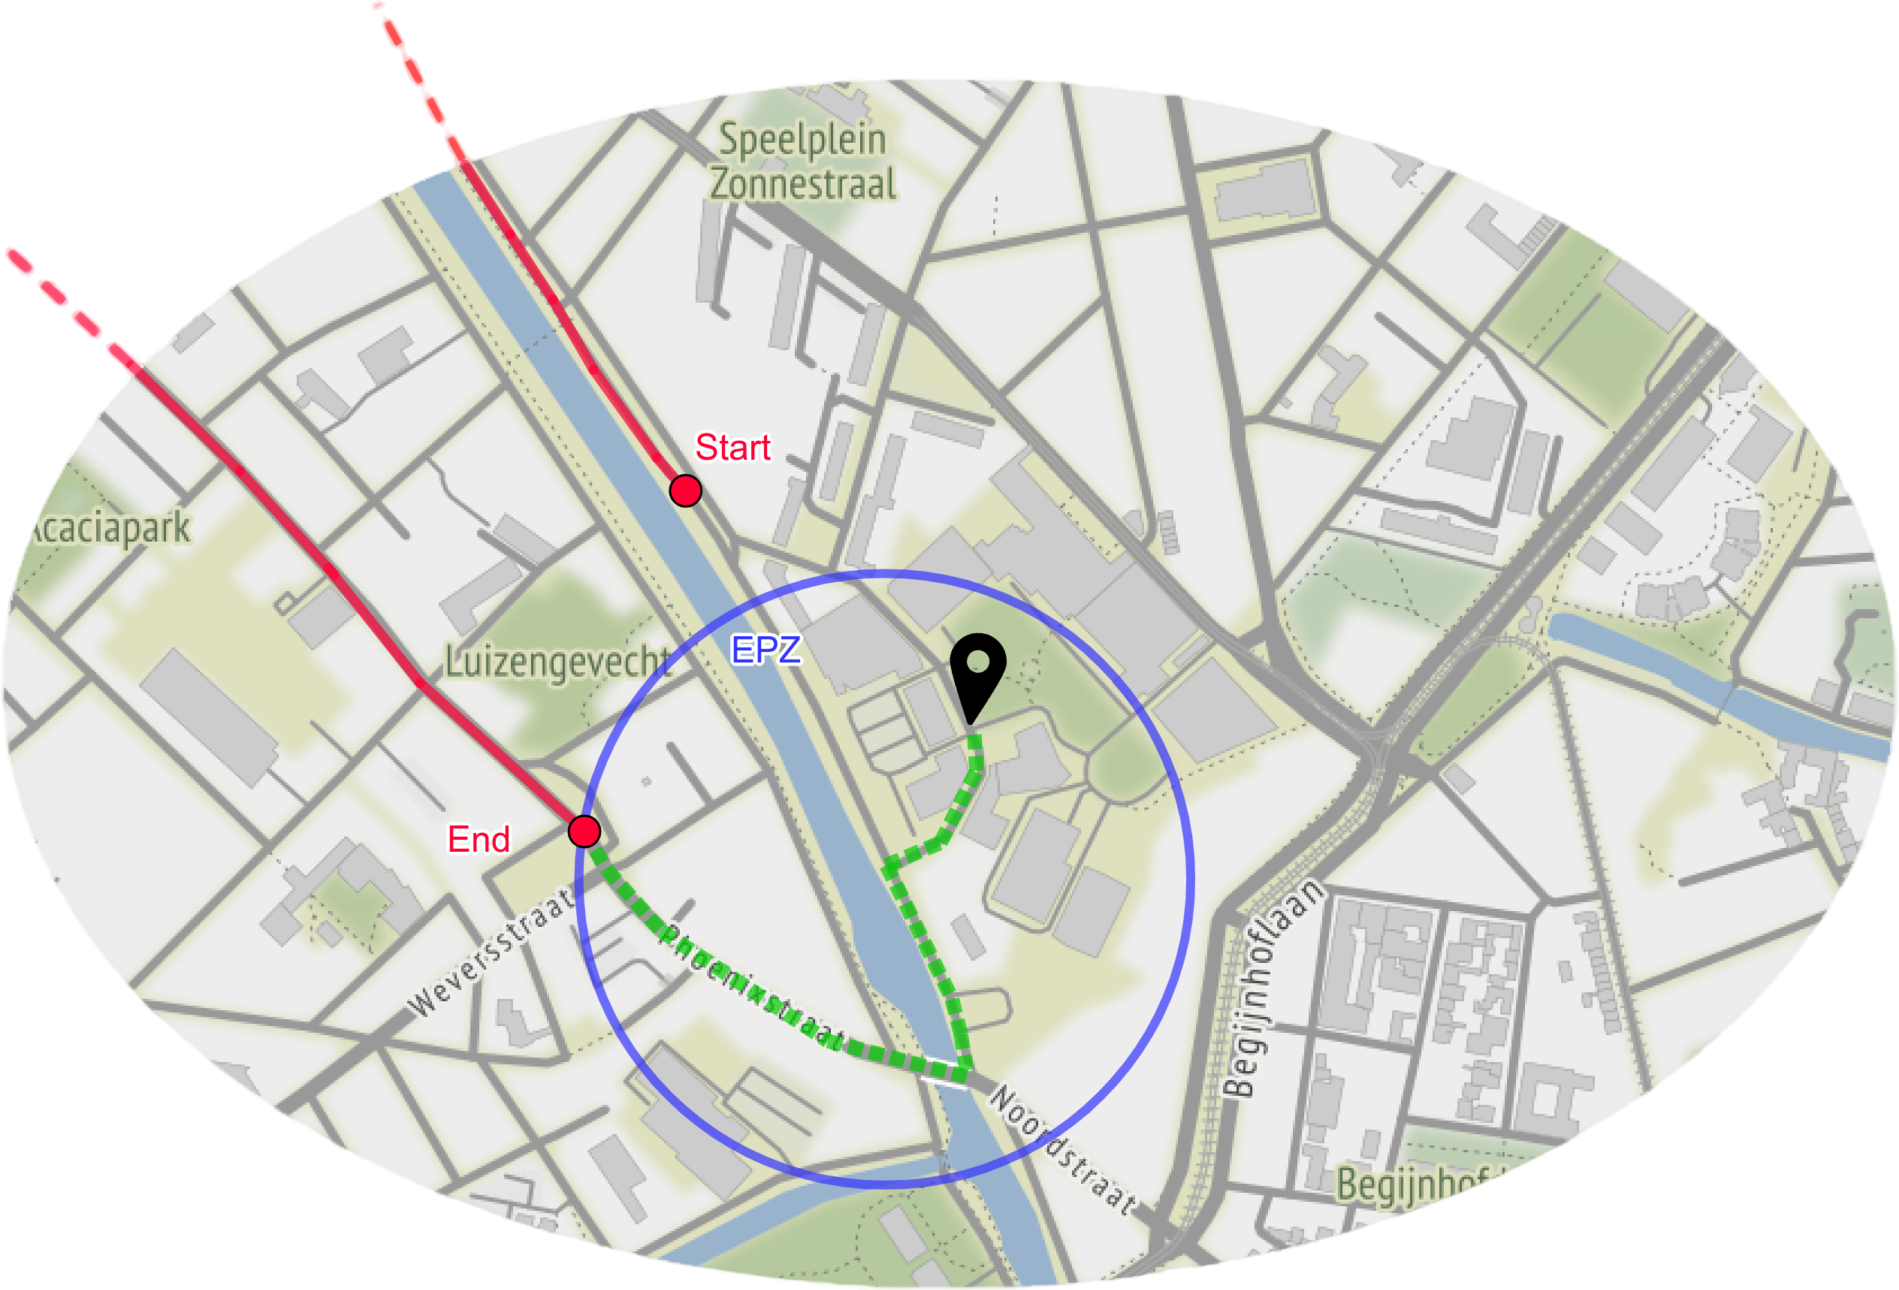
\includegraphics[width=1\textwidth]{fig/TotalDistanceAttacks/end.png}
    \end{subfigure}
    \caption{Voorbeeld van de mogelijke scenarios bij een total distance attack scenario}\label{fig:totalDistanceAttack}
\end{figure}
\begin{figure}[h]
    \centering
    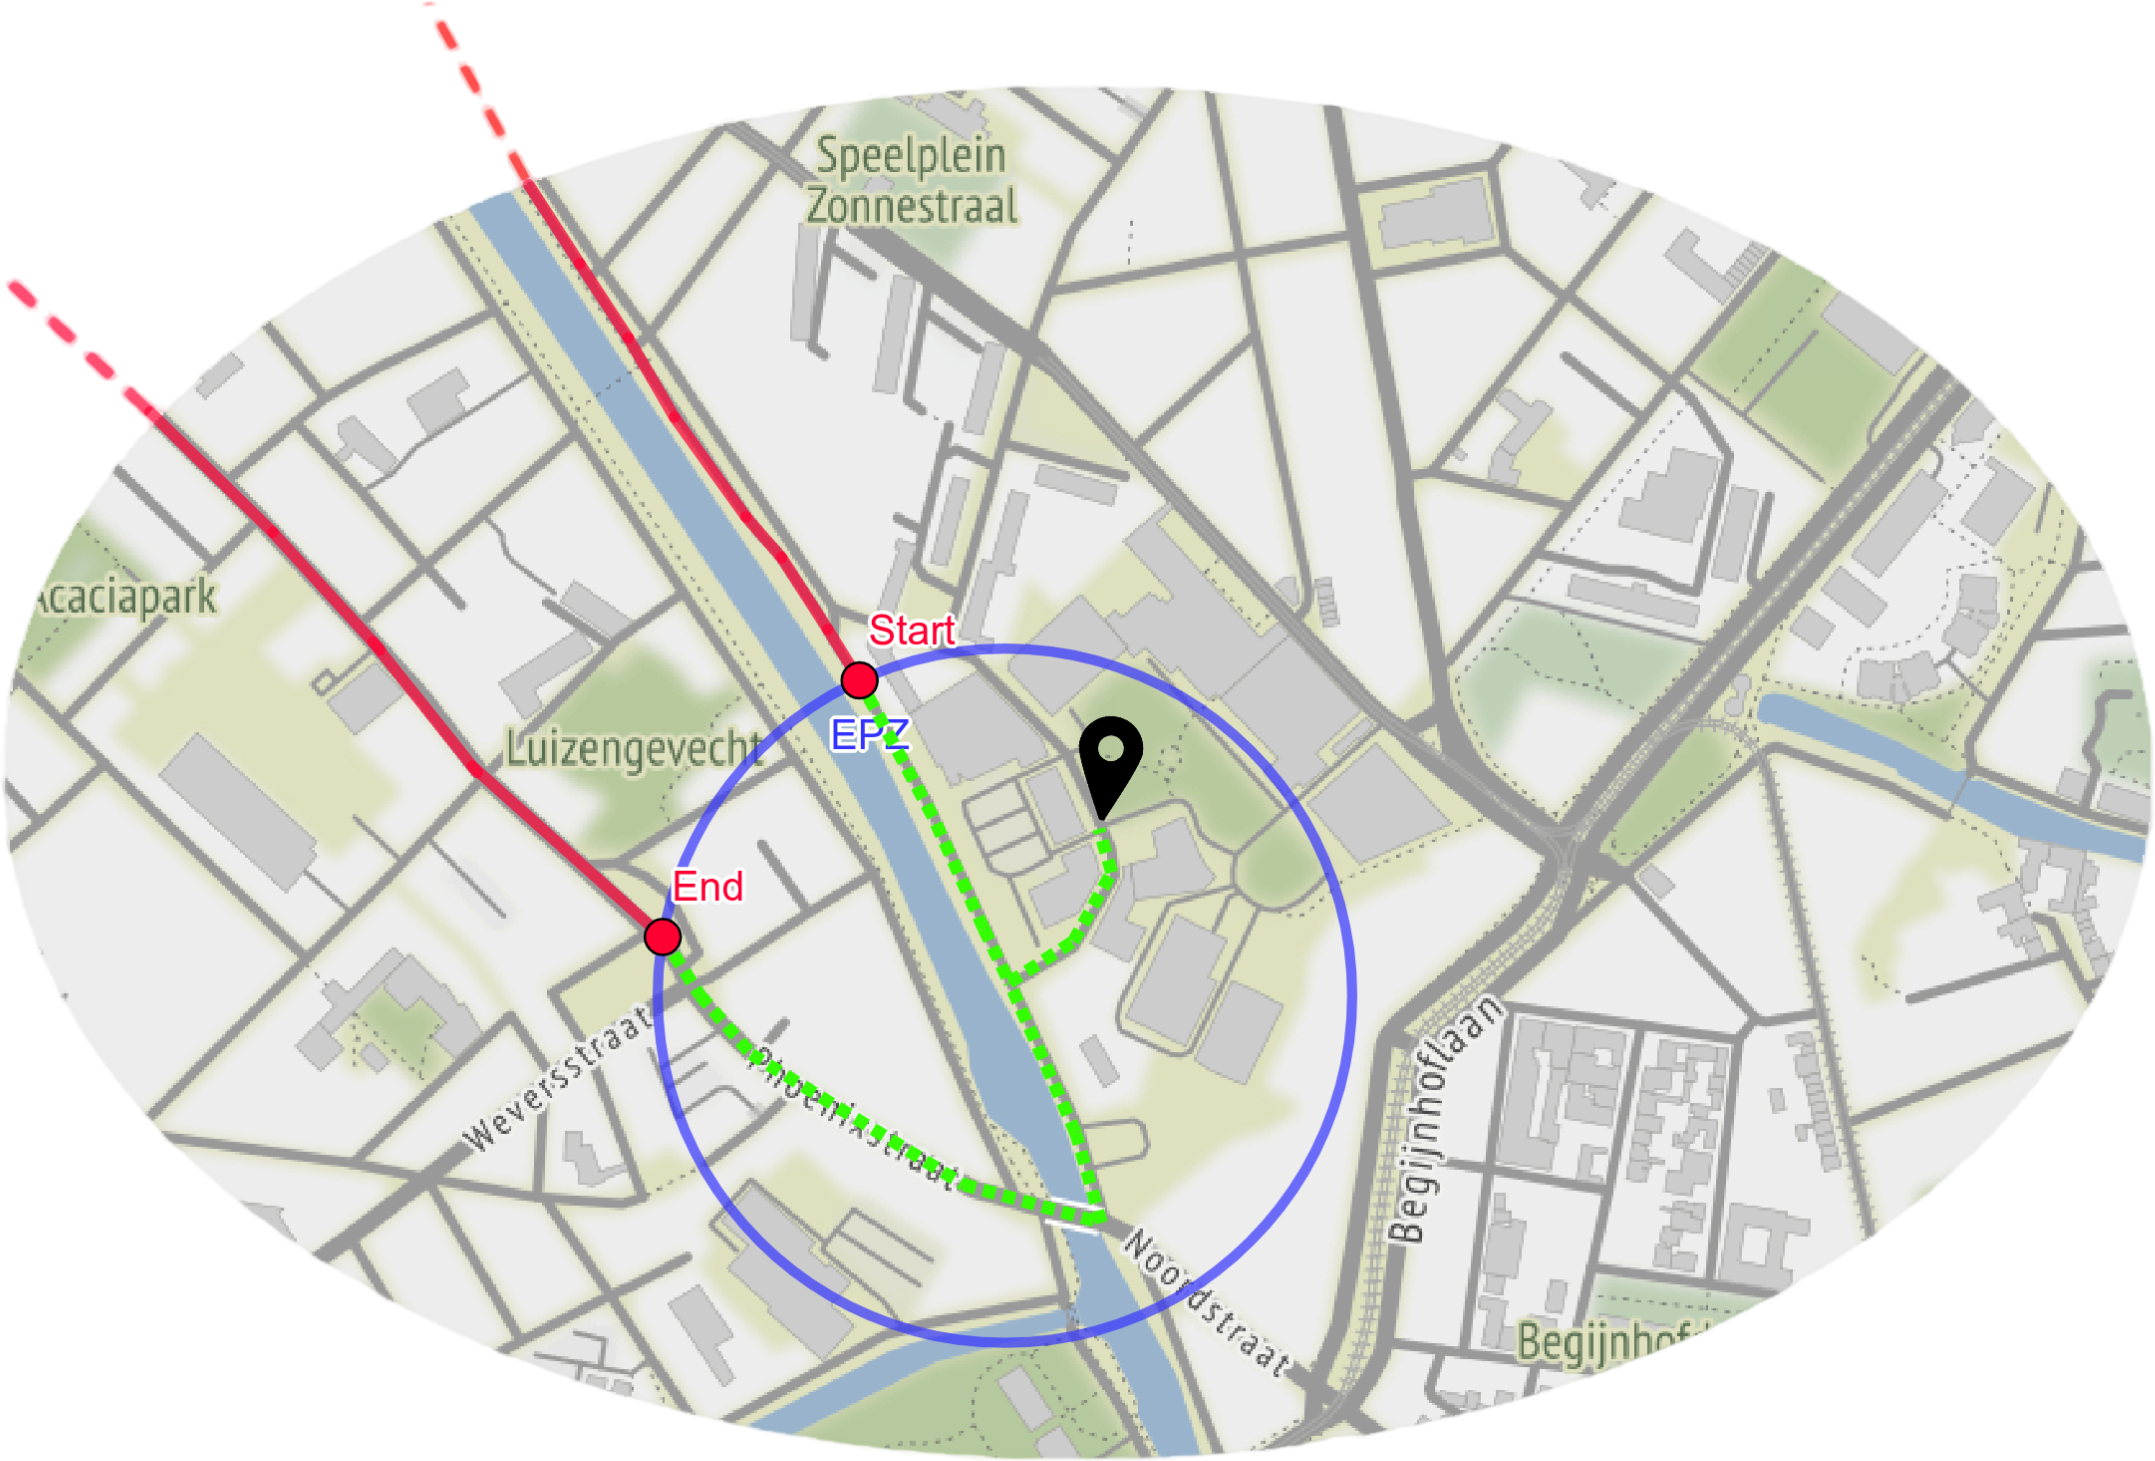
\includegraphics[width=.5\textwidth]{fig/TotalDistanceAttacks/InnerDistanceAttack.png}
    \caption{Voorbeeld van een inner distance attack situatie}\label{fig:innerDist}
\end{figure}

Deze thesis baseert zich ook voor een stuk op gemiddelde snelheden en tempo's.
Hierdoor stellen we volgende bijkomende assumptie voor: een gebruiker mag niet
stilstaan binnenin de \ac{EPZ}. Platformen zoals Strava hebben namelijk een
ingebouwde functie die bij het uploaden van een activiteit tijdstippen waarbij
een gebruiker stilstaat aan bijvoorbeeld een rood licht filtert. De gebruikers
hebben op deze manier een representatievere gemiddelde snelheid en gemiddeld
tempo. Dit wil wel zeggen dat de totale bewegingstijd waarop de gemiddelde
snelheid en tempo gebaseerd zijn, niet overeenkomt met de totale tijd van de
activiteit. Bij een berekening gebaseerd op totale verstreken tijd zou een
significante fout kunnen optreden.
% Momenteel zijn op de meeste platformen beide
% tijden afzonderlijk gegeven, maar in het theoretisch kader van dit onderzoek
% lijkt het ook nuttig om te testen in hoeverre de aanval succesvol is indien gene 

\section{Identificeren van de EPZ}
De eerste stap is het identificeren van de \ac{EPZ}. Alhoewel deze stap niet
noodzakelijk is, vernauwt deze de zoekruimte drastisch. Hierbij nemen we van
alle activiteiten die van een gebruiker ter beschikking zijn gesteld, de
zichtbare begin- en eindpunten genomen. Deze zullen dan via het k-means
algoritme worden gegroepeerd en een cirkel vormen.

K-means clustering is een unsupervised machine learning techniek die veel wordt
gebruikt bij het clusteren van data. Het is een iteratief proces waarbij het
algoritme $k$ clusters tracht te creëren waarbij de datapunten in elke cluster
zo dicht mogelijk bij het gemiddelde van die cluster
liggen~\cite{Understa24:online}. Dit algoritme kiest willekeurig initiële
middelpunten voor de verschillende clusters. Daarna kent het alle punten in de
data toe aan de cluster met de laagste Euclidische afstand tot het centrum van
deze cluster. Daarna herberekent het algoritme de gemiddeldes van deze
clusters, en worden deze gemiddeldes gezien als nieuwe centrums. Opnieuw zal
het alle punten aan de correcte cluster toekennen, en het proces herhaald zich
verschillende iteraties op deze manier. Op Figuur~\ref{fig:kmeans} is te zien
hoe de clustering bij elke iteratie beter wordt.
\begin{figure}[h]
    \centering
    \begin{subfigure}[b]{.33\textwidth}
        \centering
        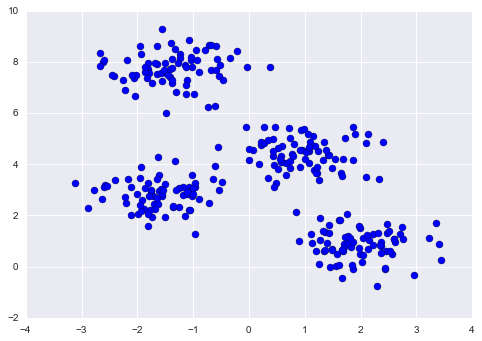
\includegraphics[width=1\textwidth]{fig/kmeans/1.png}
    \end{subfigure}\hfill
    \begin{subfigure}[b]{.33\textwidth}
        \centering
        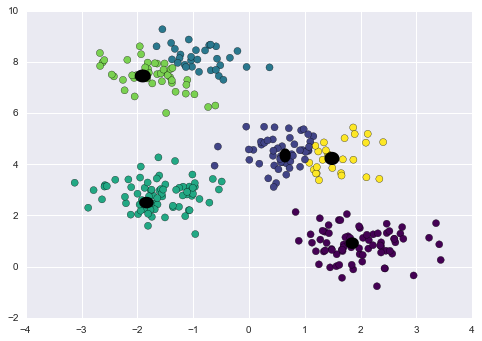
\includegraphics[width=1\textwidth]{fig/kmeans/2.png}
    \end{subfigure}
    \begin{subfigure}[b]{.33\textwidth}
        \centering
        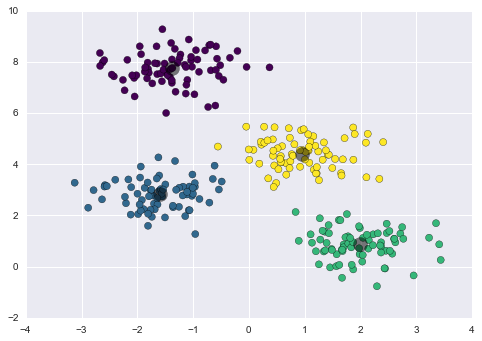
\includegraphics[width=1\textwidth]{fig/kmeans/3.png}
    \end{subfigure}
    \caption{Voorbeeld werking k-means clustering~\cite{InDepthk59:online}}\label{fig:kmeans}
\end{figure}

In de context van het identificeren van de \ac{EPZ} gebruiken we k-means om
\ac{gps}-punten te groeperen op basis van hun locaties. In plaats van te werken
met een centraal punt, werkt onze implementatie met een cirkelvormige zone, wat
zichtbaar is op Figuur~\ref{fig:kmeans_circle}. De euclidische afstand zullen
we in dit geval berekenen ten opzichte van de rand van deze cirkel. Bij elke
iteratie beschouwen we een nieuwe cirkel, en berekenen we de afstanden opnieuw.
We herhalen het proces totdat een stabiele cirkel bekomen wordt. Een cirkel is
stabiel wanneer het verschil in afstand tussen twee opeenvolgende gevonden
cirkels kleiner is dan een drempelwaarde, in dit geval 10 meter~\cite{Dhondt,
    Verdonck_2022}.
\begin{figure}[h]
    \centering
    \begin{subfigure}[b]{0.49\linewidth}
        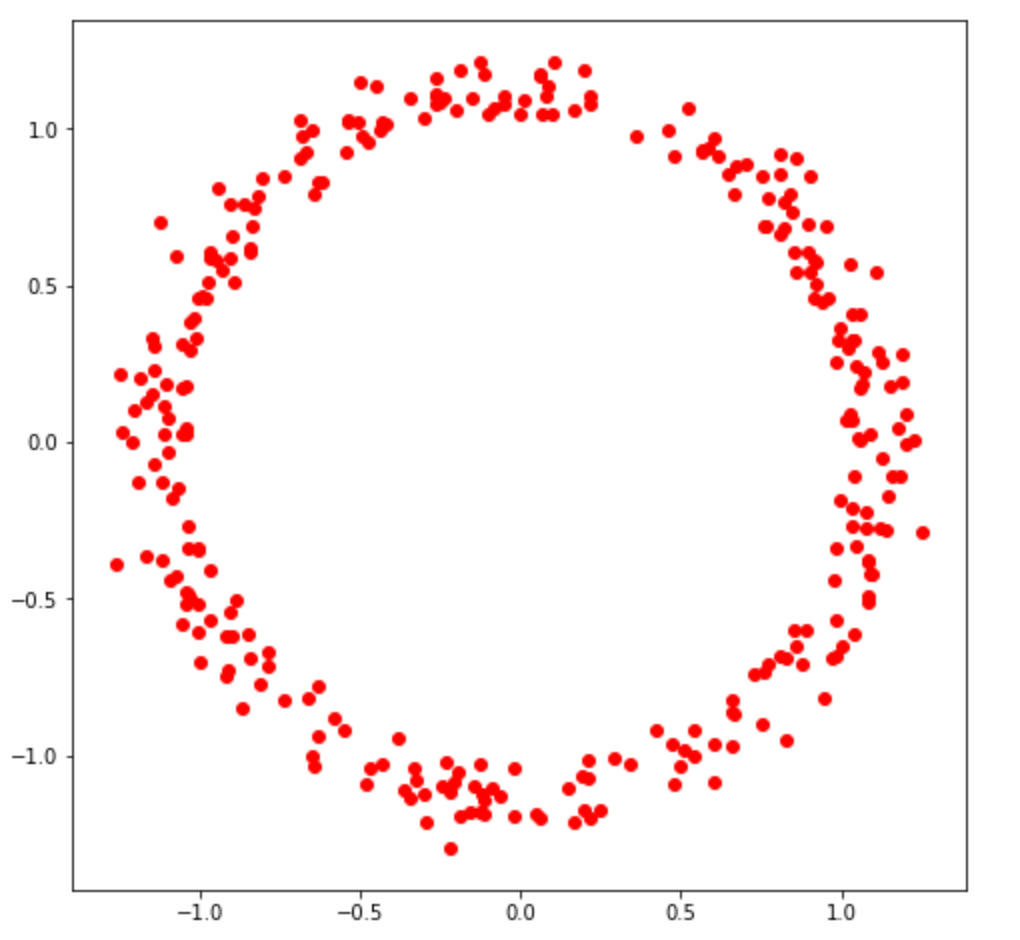
\includegraphics[width=\linewidth]{fig/kmeans/kmeans_circle.png}
    \end{subfigure}
    \begin{subfigure}[b]{0.49\linewidth}
        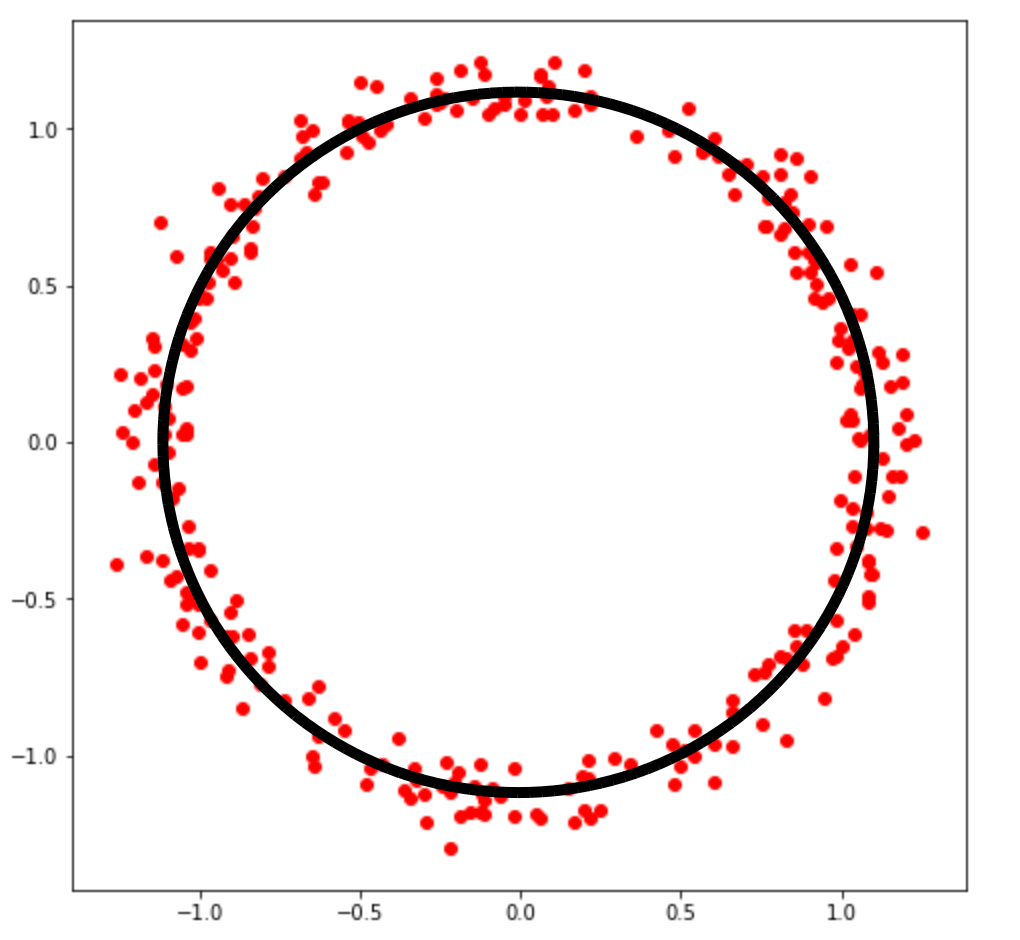
\includegraphics[width=\linewidth]{fig/kmeans/kmeans_circle copy.png}
    \end{subfigure}
    \caption{Example of datapoints which can identify a circle~\cite{DensityE3:online}}\label{fig:kmeans_circle}
\end{figure}

Het algoritme zal na de identificatie van een \ac{EPZ} ook nog nakijken of er
niet meer dan één \ac{EPZ} te vinden is. Het onderzoekt of punten die
meegenomen zijn in de beschouwing van de huidige \ac{EPZ}, toch niet horen bij
een mogelijks andere \ac{EPZ} van de user. Als controle berekent het van elk
eind- of beginpunt de Euclidische afstand tot de rand van de bijhorende
gevonden \ac{EPZ}. Indien deze kleiner is dan de grootst mogelijke radius, dan
veronderstellen we dat het punt bij deze zone hoort. Indien dit voor alle
punten geldt, dan stopt het algoritme hier. In het andere geval waarbij de
berekende afstand groter is, worden meer clusters toegevoegd aan het algoritme
van k-means clustering. Dit zal dus een nieuwe privacy zone aanwijzen.

Deze stap is niet noodzakelijk in het globale verhaal van de thesis, maar is
wel een stap die de zoekruimte drastisch kan verkleinen. Indien het algoritme
één of meerdere \acp{EPZ} vindt, dan zullen er enkel en alleen voorspellingen
gebeuren in de regio binnenin de geïdentificeerde zone. Indien dit niet het
geval is en er geen \ac{EPZ} gevonden is, bestaat de kans dat voorspellingen
van locaties gebeuren buiten de verhullende zone. Ook is in dit geval een
groter stuk van het stratennetwerk nodig om de locatie te achterhalen.

\section{Identificatie Entry Gates}
Entry gates zijn zoals de naam al doet vermoeden de `toegangspoorten' tot de
\ac{EPZ}. Dit zijn de `zones' waar de gebruiker de \ac{EPZ} kan betreden en/of
verlaten. Deze vormen zich dan ook rond wegen die de \ac{EPZ} betreden. Op
Figuur~\ref{fig:entrygate} is te zien dat meerdere eindpunten van activiteiten
geclusterd worden en een \ac{E.G.} vormen. Dit is van belang belangrijk bij het
filteren van afwijkende activiteiten. De detectie ervan gebeurt via het
\ac{DBSCAN}-algoritme.
\begin{figure}
    \centering
    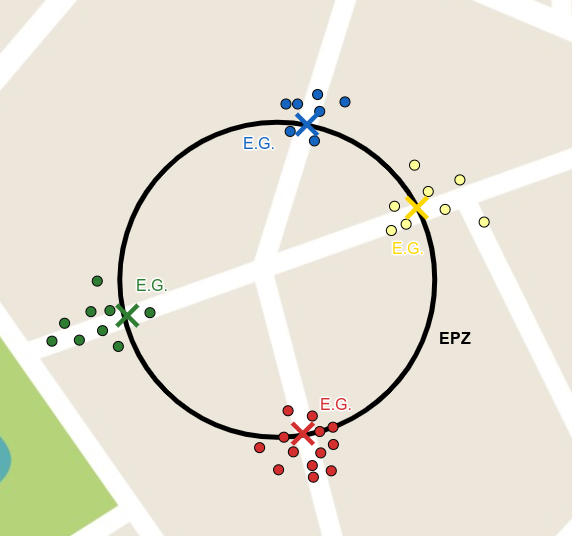
\includegraphics[width=0.5\linewidth]{fig/EPZ-mechanisme/Entry_Gate.png}
    \caption{Voorbeeld van entry gates gevonden door k-means clustering en de identificatie van een EPZ}\label{fig:entrygate}
\end{figure}

\ac{DBSCAN} is een algoritme dat clusters kan vinden in een dataset. Het vindt
clusters op basis van hun dichtheid~\cite{KMeansvs80:online}. In tegenstelling tot het eerder besproken
k-means clustering algoritme dat gebaseerd is
op het vinden van de geometrische centra van clusters, richt \ac{DBSCAN}
zich op het vinden van gebieden met een hoge dichtheid van punten.\ \ac{DBSCAN}
heeft als voordeel dat het goed overweg kan met uitschieters, want in deze
context erg nuttig blijkt. Het werkt als volgt:
\begin{enumerate}
    \item Selecteer een willekeurig niet-bezocht punt uit de set van zichtbare begin- en
          eindpunten.
    \item Bepaal of het punt een kernpunt is door te controleren of er binnen een
          bepaalde afstand een minimum aantal punten aanwezig is. Als dit het geval is,
          wordt het punt als een kernpunt beschouwd en wordt een nieuwe cluster gestart.
    \item Breid de cluster uit door alle punten binnen deze afstand van het kernpunt toe
          te voegen aan de cluster. Herhaal dit proces voor alle punten in de buurt
          totdat er geen nieuwe punten meer kunnen worden toegevoegd.
    \item Ga door naar het volgende niet-bezochte punt en herhaal de stappen 2 en 3
          totdat alle punten in de dataset zijn bezocht.
    \item Punten die niet tot een cluster behoren en niet voldoen aan de criteria voor
          kernpunten, worden beschouwd als ruispunten.
\end{enumerate}
Het algoritme maakt gebruik van twee op voorhand vast te leggen parameters: de maximale afstand tussen twee
punten in eenzelfde cluster, wat in deze context vastgelegd is op 22.9 meter en
een minimaal aantal punten dat de cluster moet bevatten, in dit geval één punt.

\section{Bepalen nodige gegevens voor predictie}
Na het bepalen van de \acp{EPZ} van de gebruiker gaan we over tot het berekenen
en achterhalen van de bijhorende gegevens die nodig zijn om de gevoelige
locatie te voorspellen. Hiervoor wordt verder ingegaan op de methodiek
beschreven inferentieaanval door~\citeauthor{Dhondt}, maar er worden enkele
gegevens op een andere manier benaderd volgens de huidige definitie van de
aanvaller.

\subsection{Roadgraph en Distance Matrix}\label{sec:roadgraph}
Voor elke gevonden EPZ is het noodzakelijk om een graafvoorstelling van de
omgeving op te stellen. Op Figuur~\ref{fig:graph_generation} is een voorbeeld
terug te vinden van hoe een graaf kan worden geëxtraheerd. Er worden punten
geplaatst op de straten op een vaste afstand van
elkaar\footnote{\label{fn:roadgraph}Op de Figuur~\ref{fig:graph_generation}
    zijn de afstanden niet altijd gelijk. De figuur is enkel nuttig ter
    illustratie, en is geen perfecte representatie de werkelijkheid.}, en deze
kunnen dan worden verbonden. Indien geen \acp{EPZ} geïdentificeerd zijn, nemen
we een ruime omgeving die we omzetten naar een graaf. De graafvoorstelling
bestaat uit een serie van nodes, die zich allemaal op een gekende straat
bevinden. De bogen waarmee de nodes verbonden zijn volgen het straatplan, opdat
een boog een mogelijks te volgen weg is~\cite{neira2022graph}. Aan de hand van
de `Chaining Distance' wordt bepaald hoeveel afstand tussen de nodes zal
zitten, en zo dus impliciet ook welke densiteit het netwerk zal hebben. Hoe
lager de chaining distance, hoe meer nodes, en dus ook hoe preciezer de
graafvoorstelling zal zijn. Om voorspellingen te maken is wel een bepaalde
precisie vereist, dus mag deze waarde niet te hoog zijn. Empirisch koos
\citeauthor{Dhondt} voor een waarde van $3.0$ meter.
\begin{figure}[h]
    \caption{Voorbeeld van het genereren van een roadgraph\footref{fn:roadgraph}}\label{fig:graph_generation}
    \centering
    \begin{subfigure}[b]{.4\textwidth}
        \centering
        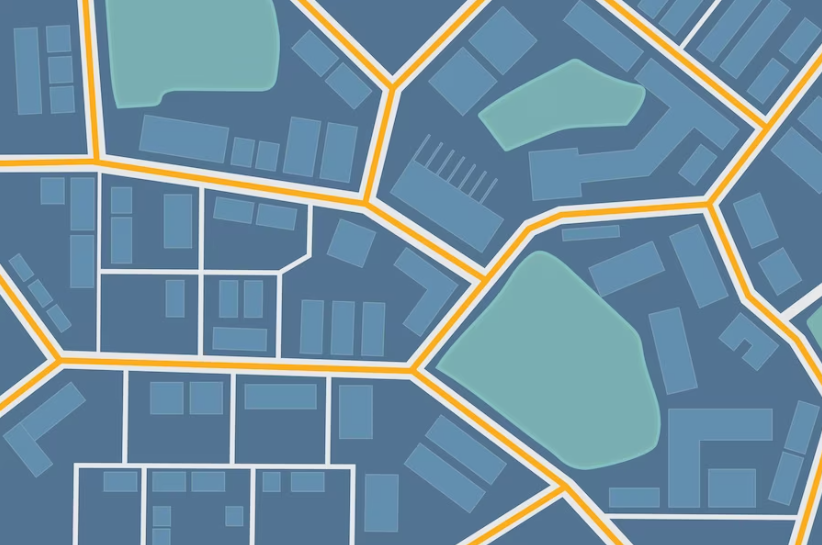
\includegraphics[width=1\textwidth]{fig/RoadGraph/RoadMap.png}
        \caption{Voorbeeld stratenplan}
    \end{subfigure}\hfill
    \begin{subfigure}[b]{.4\textwidth}
        \centering
        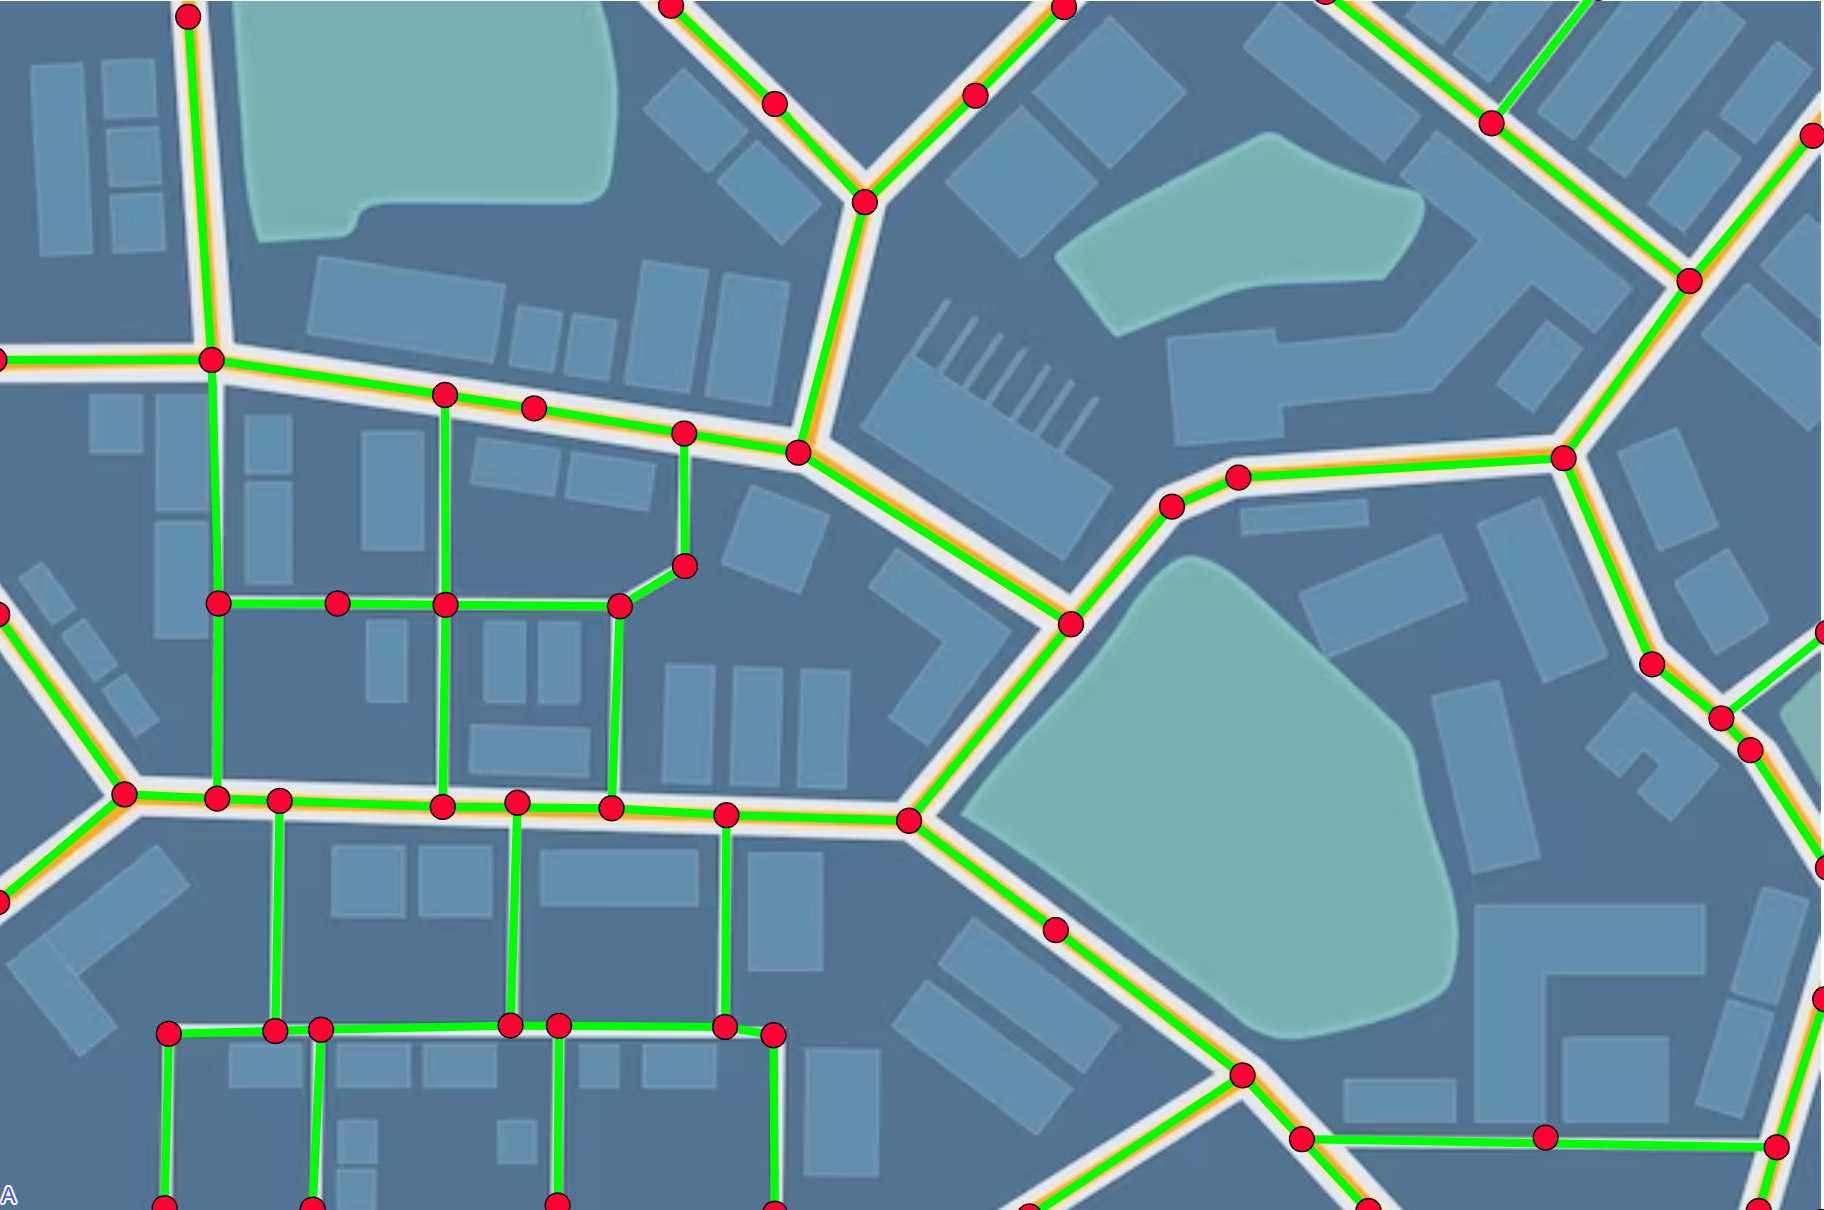
\includegraphics[width=1\textwidth]{fig/RoadGraph/Graph_Over_Map.png}
        \caption{Nodes en bogen geplot op het stratenplan}
    \end{subfigure}
    \begin{subfigure}[b]{.4\textwidth}
        \centering
        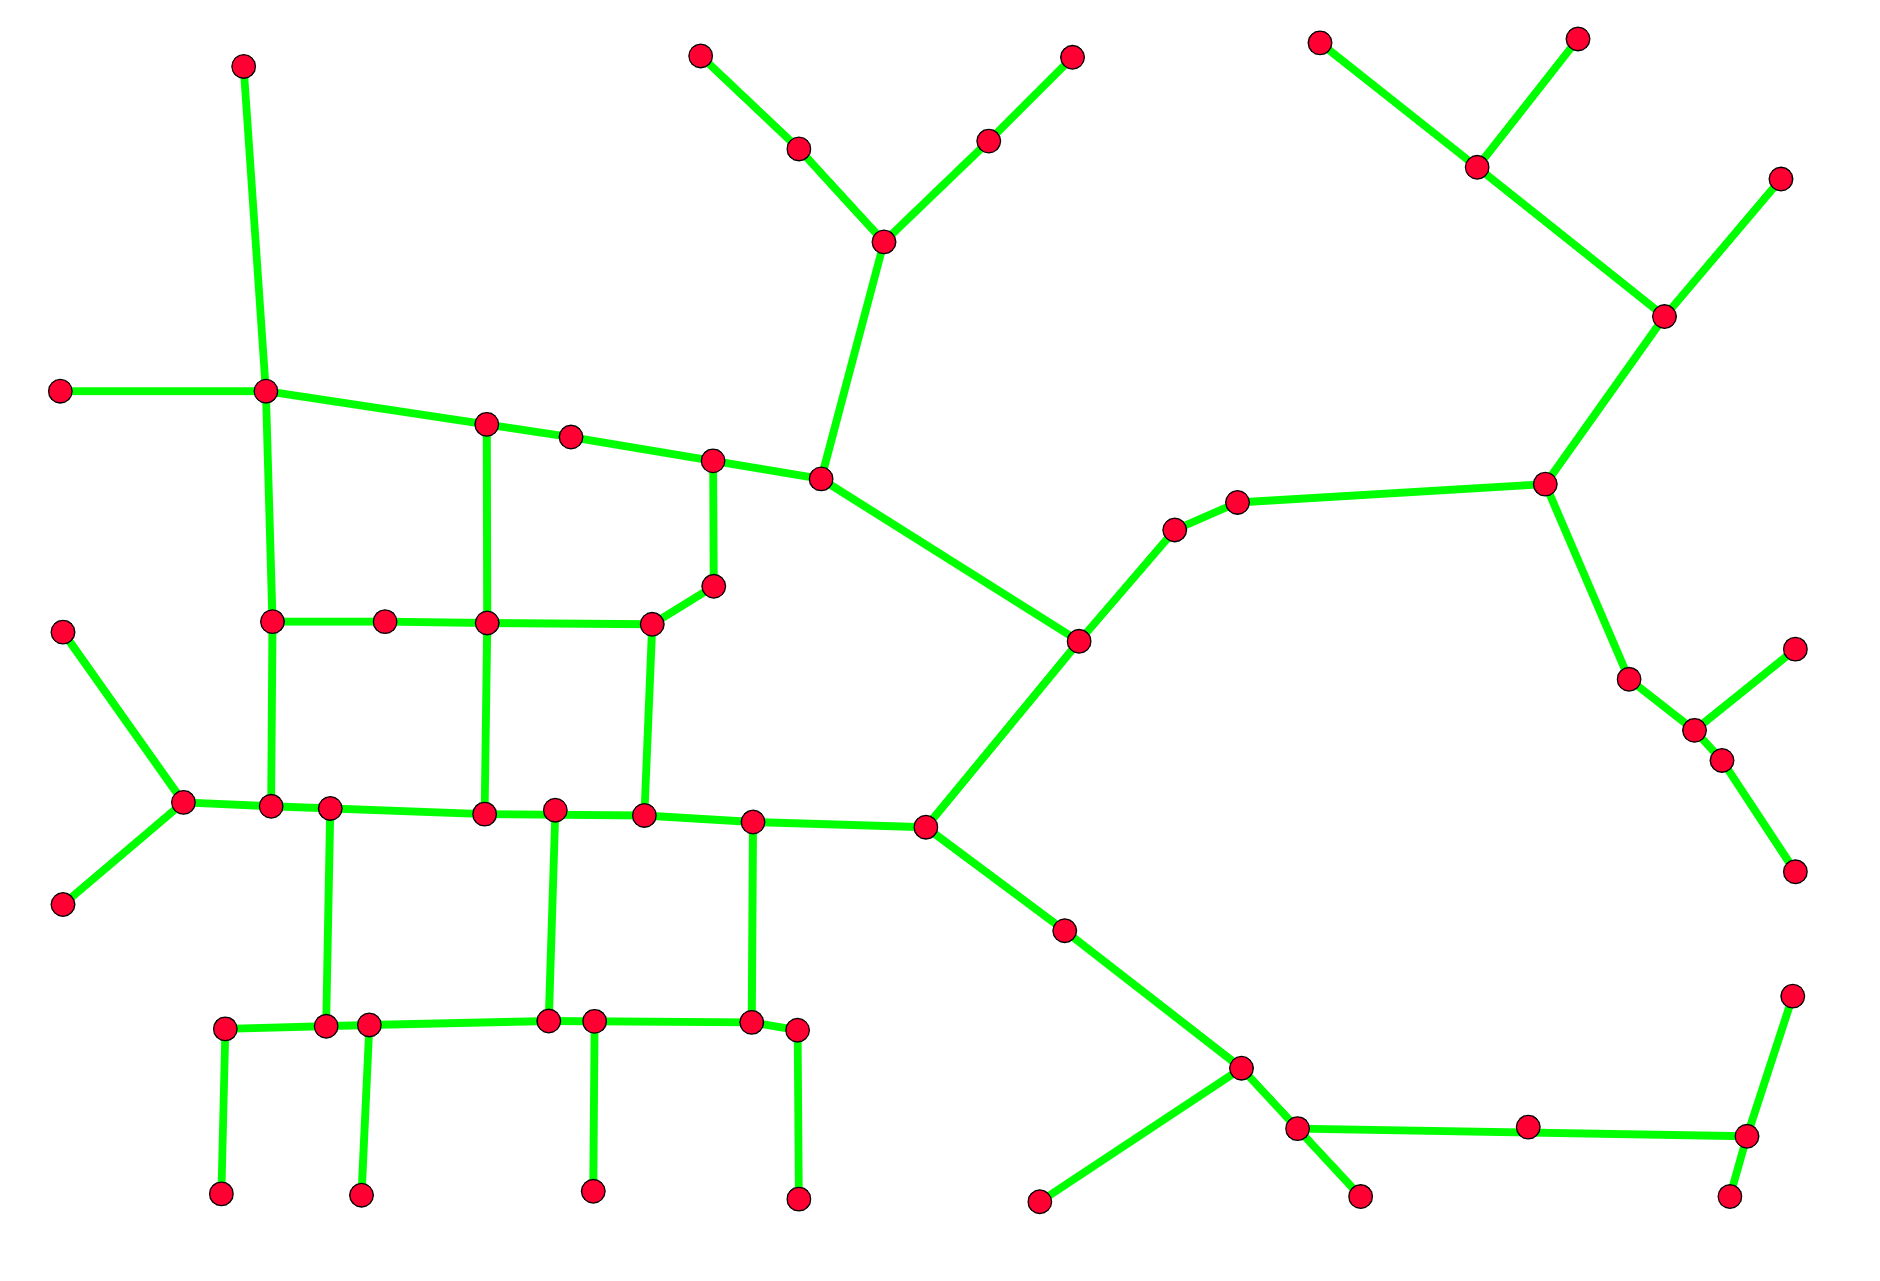
\includegraphics[width=1\textwidth]{fig/RoadGraph/Graph.png}
        \caption{Resulterende graafvoorstelling van het stratenplan}
    \end{subfigure}
\end{figure}

Op basis van de nodes in deze graaf, kan de \textit{Distance Matrix} worden
opgesteld. Dit is een matrix die voor alle startnodes (op de rand van de
\ac{EPZ}) de theoretische afstand bevat tot alle nodes aanwezig in de graaf.
Gebruikmakend van het Dijkstra algoritme\footnote{Het Dijkstra-algoritme is een
    algoritme in de grafentheorie dat wordt gebruikt om de kortste weg te vinden
    tussen twee knooppunten in een gewogen grafiek~\cite{dijkstra}. Het algoritme
    werkt door iteratief knooppunten toe te voegen aan een `bezochte' set en de
    kortste afstand te berekenen vanaf het beginpunt naar elk aangrenzend knooppunt
    dat nog niet is bezocht.}, die het in staat stelt om voor elk punt de kortste
theoretische afstand te bepalen tot alle punten in de graaf. Deze afstanden
worden opgeslagen, en zijn belangrijk in een verder stadium van de aanval.

\subsection{Begin- en eindnodes}
Voor elke activiteit is het volledige traject buiten de \ac{EPZ} gegeven. Dit
omvat alle \ac{gps}-punten die niet verborgen zijn. De begin- en eindnodes van
het traject zijn hier van belang. Voor de duidelijkheid en de vlotheid van de
tekst zullen we naar deze punten refereren als het zichtbare beginpunt en het
zichtbare eindpunt. Volgens één van de voorafgaand gemaakt assumptie vertrekt
de sporter in de \ac{EPZ} of eindigt hij erbinnen, maar beide is geen
mogelijkheid. Dit betekent dat ofwel het reële eindpunt, ofwel het reële
beginpunt zal overeenstemmen met de gevoelige locatie. In geval dat een
gebruiker aankomt binnenin de \ac{EPZ}, en dus ook vertrekt erbuiten, starten
de berekeningen vanaf het zichtbare eindpunt. Omgekeerd geldt indien de
gebruiker vertrekt binnenin de \ac{EPZ}, worden de berekeningen gestart vanaf
het zichtbare beginpunt. Deze punten zullen in het vervolg \textit{randpunten}
genoemd worden, refererend naar de rand van de \ac{EPZ}. Deze randpunten zullen
de basis vormen voor de volgende berekeningen.

Bijhorend zijn bij de randpunten ook bepaalde extra gegevens beschikbaar. De
belangrijkste zijn de cumulatieve afstand tot dit punt\footnote{De totale
    afstand afgelegd vanaf het begin van de activiteit tot en met het punt in
    kwestie.}, en de cumulatieve tijd tot dit punt\footnote{De totale tijd afgelegd
    vanaf het begin van de activiteit tot en met het punt in kwestie.}. Bij de
aanval van Dhondt et al.\ wordt de afstand gebruikt om predicties te doen. Dit
wil dus zeggen dat deze afstand dus aan de basis zal liggen. In deze thesis
wordt ervan uitgegaan dat afstanden verborgen worden. Onder het verbergen van
afstanden wordt een onderscheid gemaakt tussen 2 scenarios: het eerste gaat
ervan uit dat de totale afstand verborgen wordt, maar de cumulatieve afstand
gegeven is. Het tweede scenario gaat ervan uit dat alle afstandsgegevens
verborgen worden. Het alternatieve type data waar dus mee zal moeten gewerkt
worden is dus \ac{gps}-data.

\subsection{Berekeningen afstand binnenin de EPZ}\label{sec:berekeningen}
Om voorspellingen te kunnen doen zullen volgens de inferentieaanval die we hier
bespreken, moeten twee belangrijke gegevens ter beschikking zijn. Met name het
straatnetwerk met de mogelijks gevolgde routes, wat werd besproken in
Sectie~\ref{sec:roadgraph}, en de afstand die wordt afgelegd binnenin de
\ac{EPZ}. Deze afstand benoemen we ook als de \textit{inner distance} (dit is
niet te verwarren met de \textit{inner ditstance attack}).

In de implementatie van~\citeauthor{Dhondt} kan de \textit{inner distance}
simpelweg berekend worden door het verschil te nemen tussen de afgelegde
afstand buiten de verhulde zone (deze noemen we de \textit{outer distance}), en
de totale afstand: \[inner\ distance = total\
    distance - outer\ distance \]

In deze thesis is er echter een tussenstap noodzakelijk. In het eerste scenario
waarbij de cumulatieve afstand gegeven is, maar de totale afstand niet, moet de
totale afstand berekend worden. Maar door de aanwezigheid van snelheids- en
tijdsgegevens kan dit via basisformules gebeuren. Gebruik makend van het
gemiddelde tempo kan de voorgaande formule worden omgevormd tot: \[inner\ distance = total\ time \times average\ speed - outer\ distance \]

In opzicht van het tweede scenario, waarbij alle afstandsgegevens verborgen
zijn, ontbreekt nu ook de \textit{outer distance}. We bepalen deze via de
\ac{gps}-coördinaten. Dit gebeurd door de som te nemen van de afstanden van
tussen alle opeenvolgende punten. Let wel dat we de afstand tussen twee
\ac{gps}-punten berekenen door gebruik te maken van de \textit{haversine}
formule. Vergelijking~\ref{eq:haversine} is een uitwerking van deze
formule~\cite{sheppard1922practical}. Deze berekent de afstand tussen twee
punten op een bolvormig oppervlak, in dit geval de aarde. De breedte- en
lengtegraden van elk punt moeten omgezet worden naar radialen. Vervolgens
worden deze waarden ingevoerd in de formule, samen met de straal van de aarde
($r$), meestal genomen als $6.371 km$. De formule berekent dan de haversine
($haversine(\theta)=\sin^2(\frac{\theta}{2})$) van de helft van het verschil
tussen de breedtegraden en de haversine van de helft van het verschil tussen de
lengtegraden ($\lambda$), evenals de cosinus van de breedtegraden ($\phi$) van
beide punten. Deze waarden worden vervolgens gebruikt om de afstand tussen de
twee punten (P \& Q op Figuur~\ref{fig:haversine}) te berekenen.

Merk op dat ook dit een benadering is van de werkelijke afstand. De aarde is
niet perfect sferisch, wat de nauwkeurigheid kan beïnvloeden. Maar voor de
doeleinden binnen deze thesis is dit voldoende nauwkeurig, zeker omdat de
afstanden in deze context relatief klein zijn, waardoor over het algemeen
slechts een minimale buiging is.
\begin{equation}\label{eq:haversine}
    d = 2r \arcsin\left(\sqrt{\sin^2\left(\frac{\phi_2-\phi_1}{2}\right)+\cos(\phi_1)\cos(\phi_2)\sin^2\left(\frac{\lambda_2-\lambda_1}{2}\right)}\right)
\end{equation}
\begin{figure}[h]
    \centering
    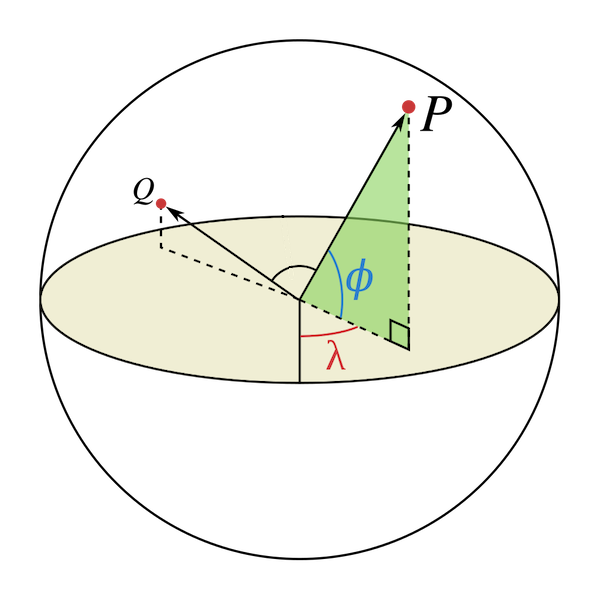
\includegraphics[width=0.5\textwidth]{fig/haversine.png}
    \caption{Haversine illustratie voor het berekenen van de afstand~\cite{Distance97:online}}\label{fig:haversine}
\end{figure}

Uit de voorgaande paragrafen kunnen we dus besluiten dat de inner distance af
te leiden valt uit gegeven outer distance, total time en de gemiddelde
snelheid. Om een \textit{outer distance attack} uit te voeren is de berekening
van de totale inner distance voldoende. Maar bij het uitvoeren van een
\textit{inner distance attack} zijn de twee afzonderlijke inner distances nodig
(degene van start tot de \ac{EPZ} en degene van de \ac{EPZ} tot de finish).
Wanneer de cumulatieve afstand gegeven is, zouden we een deze aanval kunnen
uitvoeren doordat in dit geval de twee afstanden te achterhalen zijn.
$d_{start} = d_{eerste\ node}$ en $d_{finish} = d_{totaal} - d_{laatste\
            node}$. Maar wanneer deze niet beschikbaar zijn, is dit niet mogelijk, in dit
geval zijn deze afstanden niet individueel te achterhalen.

\section{Voorspellen locatie}
Alle nodige gegevens zijn nu beschikbaar om de gevoelige locatie te
achterhalen. Hier wordt besproken hoe voor elke bruikbare activiteit een
locatie zal worden voorspeld. Doordat voor elke activiteit één of meerdere
locaties worden voorspeld, zullen we deze moeten bundelen tot één locatie voor
alle activiteiten.

\subsection{Filteren activiteiten}
Voorafgaand aan het voorspellen is het van essentieel belang om uitsluitend
voorspellingen te maken op basis van activiteiten die een waardevolle
voorspelling kunnen genereren. Andere activiteiten zouden enkel de accuraatheid
van de voorspelling naar beneden halen. Dit gaat dan bijvoorbeeld over
activiteiten waarbij niet de kortste route binnenin de \ac{EPZ} wordt gevolgd.
Al deze activiteiten proberen we dus in de mate van het mogelijke eruit te
filteren.

Het geval waarbij een gebruiker niet de kortste route volgt vanaf de rand van
de \ac{EPZ} tot de gevoelige locatie kunnen we in zekere mate opvangen door te
stellen dat we een activiteit enkel nog gebruiken wanneer de nog af te leggen
afstand binnenin de \ac{EPZ} kleiner is dan de maximaal mogelijk af te leggen
weg. In de andere gevallen zullen we de activiteit weggooien. De maximale
afstand die hiervoor nodig is wordt bepaald gebruik makend van de
\textit{Distance Matrix}, die beschreven staat in Sectie~\ref{sec:roadgraph}.
De maximale afstand is gelijk aan de maximale afstand terug te vinden in de
matrix, voor de bijhorende startnode. Dit is de afstand die een gebruiker
maximaal kan afleggen naar eender welke node op de graaf, vertrekkend van de
startnode, door het volgen van de theoretisch kortste route. Dit zal ook
gevallen in rekening brengen waarbij het traject voor een stuk verborgen wordt,
maar niet zal eindigen op de gevoelige locatie.

Op een gelijkaardige manier kan een filtering gebeuren voor afgelegde afstanden
die lager zijn dan de minimale mogelijke afstand. Dit zou opnieuw activiteiten
kunnen filteren die niet eindigen op de gevoelige afstand. De minimale afstand
is dan ook degene tot de node met de laagste minimale afstand tot deze node
vanaf het zichtbare startpunt of eindpunt van de activiteit, gelegen op de rand
van de \ac{EPZ}.

Om de zichtbare eind- en beginpunten van de activiteiten te controleren op
compatibiliteit met de road graph, voeren we een actieve verificatie uit.
Hierbij worden alle eind- en beginpunten op de graaf `gesnapt', ofwel vervangen
door de dichtstbijzijnde knooppunt op de graaf. We berekenen de afstand tussen
de oorspronkelijke locatie en de gesnapte locatie. Indien het verschil in
afstand te groot is, filteren we de betreffende activiteit. Een aanzienlijk
verschil in afstand kan duiden op een afwijking tussen de gevolgde route en de
road graph, of op onnauwkeurige gps-gegevens.

Als laatste wordt nog gekeken naar afwijkingen bij de \acp{E.G.}. Indien bij
een activiteit een afwijking wordt vastgesteld tussen de zichtbare begin- en
eindpunten en de \ac{E.G.} die groter is dan drie maal de standaardafwijking,
wordt de activiteit gefilterd. Dit wijst dan op een te grote spreiding bij ten
opzichte van de \ac{E.G.}, en dus op een grote kans op inaccurate
voorspellingen.

\subsection{Bepalen van de locatie}
Om een predictie te maken per activiteit wordt de inner distance die berekend
werd in Sectie~\ref{sec:berekeningen} gebruikt. Deze wordt dan gematched met
het stratennetwerk. Het idee hierachter is om alle mogelijke routes (die de
kortste route vormt naar alle nodes op zijn pad) binnenin de \ac{EPZ} af te
leggen, en te stoppen wanneer de afgelegde afstand gelijk is aan de berekende
inner distance. Het resultaat van deze gevolgde route is dan een node, die
mogelijks de gevoelige locatie kan voorstellen. In de praktijk kunnen we dit
mechanisme op een simpele manier toepassen door gebruik te maken van de vooraf
berekende distance matrix. De berekende inner distance zal worden vergeleken
met de afstanden in de distance matrix.

Deze methodiek herhalen we voor elke activiteit die niet werd gefilterd. Al
deze voorspellingen worden uiteindelijk gebundeld tot één voorspelling in de
volgende stap.

\subsection{Regressie om te komen tot een eindvoorspelling}\label{sec:lad}
Om de routes die we in vorige sectie bepaalden om te vormen tot één
eindvoorspelling, voeren we een regressie-analyse uit, aan de hand van de
\ac{LAD} methode. Het resultaat van deze regressie-analyse zal een
\ac{gps}-locatie zijn, die onze \textit{eindvoorspelling} zal vormen.

De \ac{LAD} methode wordt gebruikt om een lineaire regressie uit te voeren op
een set punten, door de som van de absolute waarden van de absolute verschillen
te minimaliseren.\ \ac{LAD} staat gekend als een robuuste methode die erg
nuttig blijkt te zijn voor datasets met grote uitschieters. In
Vergelijking~\ref{eq:LAD} is te zien dat, door het werken met absolute waarden,
extremen in mindere mate doorwegen in de berekeningen. Dit is een groot
voordeel ten opzichte van andere regressietechnieken, zoals
bijvoorbeeld~\ac{OLS}~\cite{iqbal2021application}.~\ac{OLS} werkt gelijkaardig,
maar zoals te zien is in Vergelijking~\ref{eq:OLS} probeert deze de som van de
kwadratische afwijkingen te minimaliseren. Uitschieters zullen dus meer
doorwegen. Een nadeel van \ac{LAD} is dat het berekenen van de LAD-schattingen
meer rekentijd en computerbronnen vereist dan \ac{OLS}, wat het minder geschikt
maakt voor grote datasets.
\begin{equation} \label{eq:LAD}
    LAD:\indent  \min\sum\limits_{i=1}^n|d_i - d_{inner}|
\end{equation}
\begin{equation} \label{eq:OLS}
    OLS:\indent  \min\sum\limits_{i=1}^n{(d_i - d_{inner})}^2
\end{equation}

In deze context gebruiken we LAD regressie door de aard van de data en
voorspellingen, meer bepaald door de grote kans op uitschieters. Gps-data kan
erg onnauwkeurig zijn, en grote of kleine afwijkingen kunnen dus voorkomen. Ook
is het mogelijk dat door acties van een sporter zoals bijvoorbeeld eenmalig de
kortste route niet volgen, uitschieters voorvallen. Rekentijd is in deze thesis
geen probleem, aangezien de dataset beperkt blijft tot 100 activiteiten.

In de context van deze thesis kan Vergelijking~\ref{eq:LAD} worden toegepast
voor elke node in de graaf. Elke node in graaf zullen we individueel beschouwen
als een mogelijke eindvoorspelling. Het verschil tussen de nog af te leggen
afstand voor deze activiteit, of dus de inner distance en de theoretische
afstand tot de node vanaf het zichtbare begin- of eindpunt, wat af te lezen
valt uit de distance matrix, stelt dan de afwijking voor van deze activiteit.
Indien we dit sommeren over alle activiteiten voor dezelfde node, bekomen we
een waarde die de totale afwijking voorstelt indien we voor deze node als
eindvoorspelling zouden kiezen. We overlopen alle nodes in de graaf, en
selecteren deze met de laagste totale afwijking. Deze node zal dan de
\textbf{eindvoorspelling} voor deze activiteit voorstellen.

% Alle voorspelde locaties zullen worden beschouwd als mogelijke
% \textit{eindvoorspelling}. Deze zal dan in de vergelijking $\hat{y}$
% voorstellen. De absolute waarde van het verschil tussen de eindvoorspelling en
% alle overige punten zal worden opgeteld. Er wordt gezocht naar het punt waarbij
% de som van de absolute waarde minimaal is, en dit is dan de resulterende
% predictie, de \textbf{eindvoorspelling}.

% Apart hoofdstuk voor de setting en de aanval zelf